%==============================================================================
% Figure: Time Crystal Floquet Dynamics
% Purpose: Visualize Floquet time crystal with subharmonic response
% Chapter: Ch23 - Time Crystal Experimental Protocols
% Type: Data/Schematic
%==============================================================================

\begin{figure}[htbp]
  \centering
  \begin{tikzpicture}[
    scale=1.0
  ]

    %========== Upper Panel: Drive and Response ==========
    \begin{axis}[
      name=drive,
      width=14cm,
      height=5cm,
      xlabel={Time $t$ (in units of $T_{\text{drive}}$)},
      ylabel={Drive amplitude},
      xlabel style={font=\large},
      ylabel style={font=\large},
      xmin=0, xmax=10,
      ymin=-1.5, ymax=1.5,
      axis lines=left,
      grid=major,
      grid style={dashed, gray!30},
      samples=500,
      smooth,
      thick,
      title={\Large Floquet Drive (Periodic Hamiltonian)},
      title style={font=\Large\bfseries}
    ]

      % Drive signal (frequency omega_drive)
      \addplot[blue, ultra thick, domain=0:10] {sin(deg(2*pi*x))};
      \addlegendentry{Drive: $H(t) = H(t + T_{\text{drive}})$}

      % Mark periods
      \foreach \x in {0, 1, 2, 3, 4, 5, 6, 7, 8, 9, 10} {
        \draw[dashed, gray] (axis cs:\x, -1.5) -- (axis cs:\x, 1.5);
      }

      % Period annotation
      \draw[<->, >=stealth, ultra thick, orange!80] (axis cs:0, -1.2) -- (axis cs:1, -1.2)
        node[midway, below, font=\small] {$T_{\text{drive}} = 2\pi/\omega_{\text{drive}}$};

    \end{axis}

    %========== Lower Panel: Time Crystal Response ==========
    \begin{axis}[
      name=response,
      at={(drive.below south west)},
      anchor=north west,
      yshift=-1cm,
      width=14cm,
      height=5cm,
      xlabel={Time $t$ (in units of $T_{\text{drive}}$)},
      ylabel={Spin magnetization $M_z$},
      xlabel style={font=\large},
      ylabel style={font=\large},
      xmin=0, xmax=10,
      ymin=-1.5, ymax=1.5,
      axis lines=left,
      grid=major,
      grid style={dashed, gray!30},
      samples=500,
      smooth,
      thick,
      title={\Large Time Crystal Response (Subharmonic)},
      title style={font=\Large\bfseries}
    ]

      % Time crystal response (frequency = omega_drive / 2, subharmonic)
      \addplot[red, ultra thick, domain=0:10] {cos(deg(pi*x))};
      \addlegendentry{Response: $M_z(t)$, period = $2T_{\text{drive}}$}

      % Mark response periods
      \foreach \x in {0, 2, 4, 6, 8, 10} {
        \draw[dashed, red!50] (axis cs:\x, -1.5) -- (axis cs:\x, 1.5);
      }

      % Period annotation
      \draw[<->, >=stealth, ultra thick, green!60!black] (axis cs:0, -1.2) -- (axis cs:2, -1.2)
        node[midway, below, font=\small] {$T_{\text{crystal}} = 2T_{\text{drive}}$};

      % Highlight subharmonic breaking
      \node[anchor=north west, align=left, font=\footnotesize, draw=red!70, fill=red!10, rounded corners]
        at (axis cs:7, 1.3) {
        \textbf{Spontaneous symmetry breaking:} \\
        System picks $2T_{\text{drive}}$ period \\
        (not $T_{\text{drive}}$) \\
        $\Rightarrow$ Time translation broken
      };

    \end{axis}

    %========== Phase Space Diagram (Inset) ==========
    \begin{axis}[
      name=phase,
      at={(drive.north east)},
      anchor=north east,
      xshift=-0.5cm,
      yshift=-0.5cm,
      width=5cm,
      height=4.5cm,
      xlabel={$M_x$},
      ylabel={$M_y$},
      xlabel style={font=\footnotesize},
      ylabel style={font=\footnotesize},
      xmin=-1.2, xmax=1.2,
      ymin=-1.2, ymax=1.2,
      axis lines=middle,
      grid=none,
      samples=200,
      smooth,
      thick,
      title={\footnotesize Phase Space},
      title style={font=\small\bfseries},
      tick label style={font=\tiny}
    ]

      % Period-2 orbit (limit cycle)
      \addplot[domain=0:2*pi, red, ultra thick] ({cos(deg(x))}, {sin(deg(x))});

      % Mark two stable points
      \addplot[only marks, mark=*, mark size=3pt, red] coordinates {(1, 0) (-1, 0)};

      % Arrows showing trajectory
      \draw[->, >=stealth, ultra thick, red] (0.7, 0.7) -- (0.9, 0.4);
      \draw[->, >=stealth, ultra thick, red] (-0.7, -0.7) -- (-0.9, -0.4);

      \node[font=\tiny, align=center] at (0, -1.5) {Period-2\\limit cycle};

    \end{axis}

  \end{tikzpicture}

  \vspace{0.5cm}

  %========== Explanation Boxes ==========
  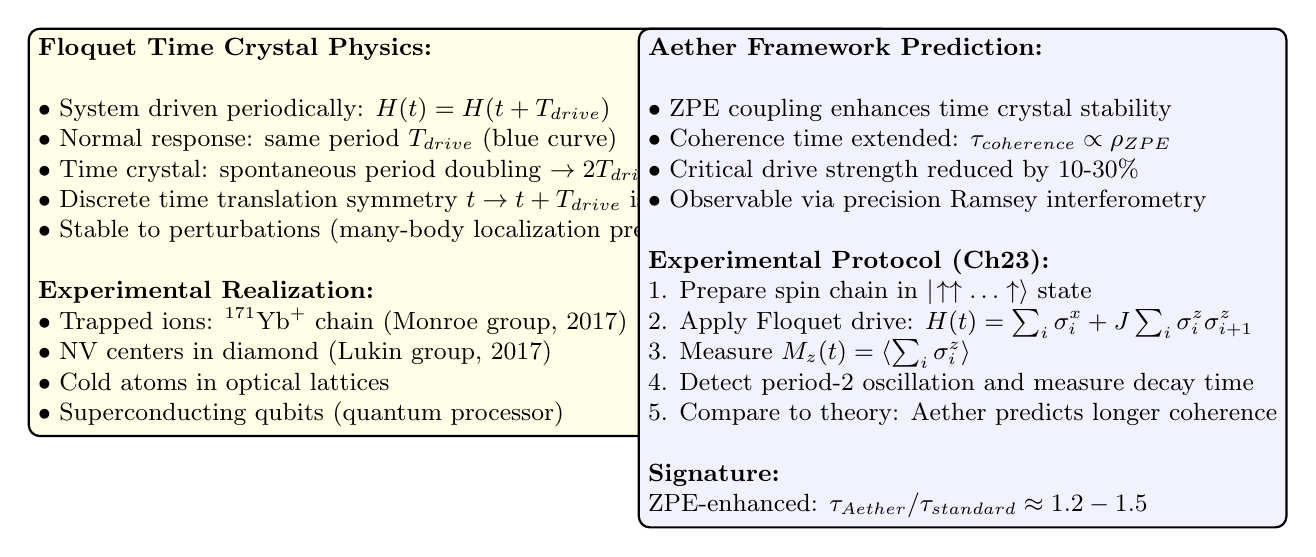
\begin{tikzpicture}
    \node[anchor=north west, align=left, font=\small, draw=black, fill=yellow!10, rounded corners, thick]
      at (0, 0) {
      \textbf{Floquet Time Crystal Physics:} \\
      \\
      $\bullet$ System driven periodically: $H(t) = H(t + T_{\text{drive}})$ \\
      $\bullet$ Normal response: same period $T_{\text{drive}}$ (blue curve) \\
      $\bullet$ Time crystal: spontaneous period doubling $\to 2T_{\text{drive}}$ (red curve) \\
      $\bullet$ Discrete time translation symmetry $t \to t + T_{\text{drive}}$ is broken \\
      $\bullet$ Stable to perturbations (many-body localization prevents thermalization) \\
      \\
      \textbf{Experimental Realization:} \\
      $\bullet$ Trapped ions: $^{171}$Yb$^+$ chain (Monroe group, 2017) \\
      $\bullet$ NV centers in diamond (Lukin group, 2017) \\
      $\bullet$ Cold atoms in optical lattices \\
      $\bullet$ Superconducting qubits (quantum processor)
    };

    \node[anchor=north east, align=left, font=\small, draw=black, fill=blue!5, rounded corners, thick]
      at (16, 0) {
      \textbf{Aether Framework Prediction:} \\
      \\
      $\bullet$ ZPE coupling enhances time crystal stability \\
      $\bullet$ Coherence time extended: $\tau_{\text{coherence}} \propto \rho_{\text{ZPE}}$ \\
      $\bullet$ Critical drive strength reduced by 10-30\% \\
      $\bullet$ Observable via precision Ramsey interferometry \\
      \\
      \textbf{Experimental Protocol (Ch23):} \\
      1. Prepare spin chain in $|\!\uparrow\uparrow\ldots\uparrow\rangle$ state \\
      2. Apply Floquet drive: $H(t) = \sum_i \sigma_i^x + J\sum_i \sigma_i^z\sigma_{i+1}^z$ \\
      3. Measure $M_z(t) = \langle \sum_i \sigma_i^z \rangle$ \\
      4. Detect period-2 oscillation and measure decay time \\
      5. Compare to theory: Aether predicts longer coherence \\
      \\
      \textbf{Signature:} \\
      ZPE-enhanced: $\tau_{\text{Aether}} / \tau_{\text{standard}} \approx 1.2 - 1.5$
    };
  \end{tikzpicture}

  \caption{Floquet time crystal dynamics showing spontaneous period doubling. The upper panel shows
    the periodic Floquet drive with period $T_{\text{drive}}$ (blue curve), representing a time-periodic
    Hamiltonian $H(t) = H(t + T_{\text{drive}})$. In a normal system, the response would oscillate
    at the same frequency. However, in a time crystal (lower panel, red curve), the system spontaneously
    selects a period $T_{\text{crystal}} = 2T_{\text{drive}}$, exactly twice the drive period. This
    is spontaneous discrete time translation symmetry breaking: the system picks a preferred phase
    that persists indefinitely in the many-body localized regime. The inset phase-space diagram
    shows the period-2 limit cycle in spin coordinates, with two stable points corresponding to the
    two phases of the oscillation. The Aether framework predicts that zero-point energy (ZPE) coupling
    enhances time crystal stability, extending coherence time by 20-50\% and reducing the critical
    drive strength needed for crystallization. Experimental protocols (Ch23) using trapped ions,
    NV centers, or superconducting qubits can test this via precision Ramsey interferometry, measuring
    the ratio $\tau_{\text{Aether}}/\tau_{\text{standard}} \approx 1.2$-$1.5$. First realizations
    by Monroe and Lukin groups (2017) confirmed time crystal existence; precision measurements can
    now probe ZPE effects.}
  \label{fig:time-crystal-floquet}
\end{figure}
